\section{Theorie}
\label{sec:Theorie}

\subsection{Allgemeine Funktionsweise}

Brückenschaltungen werden im Allgemeinen hauptsächlich zur Messung unbekannter Größen 
gebraucht, die sich eideutig auf ihren Widerstand reduzieren lassen. Darunter fallen für
die folgende Versuchsreihe Ohm'sche Widerstände, Kapazitäten von Kondenstatoren und 
Induktivitäten von Spulen. Der grundsätzliche Aufbau \ref{fig:allg} funktioniert dabei, wie folgt:
Zwischen den Stellen $C$ und $D$ wird eine Spannung abgegriffen, die von den in der Masche 
enthaltenen Widerständen abhängig ist. Anhand dessen lässt sich unter der Bedingung, dass 
nur einer der in dem Fall ohmschen Widerstände unbekannt ist, dieser über die Beziehung
von Spannung und Widerständen bestimmen. 
\begin{figure}
\centering
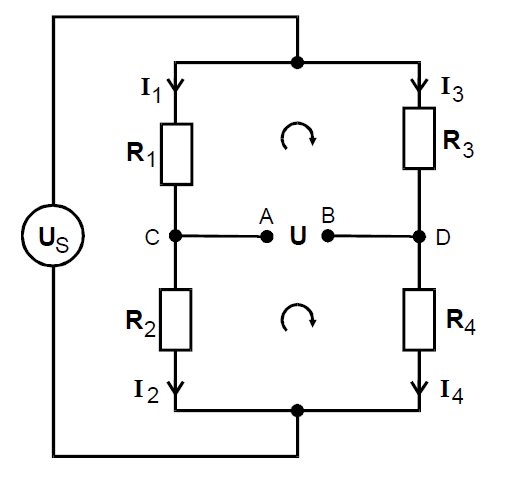
\includegraphics[width=\textwidth]{allgemeine_bs.png}
\caption{Allgemeine Brückenschaltungen}
\label{fig:allg}
\end{figure}

Um dies zu können, müssen die zwei Kirchhoff'schen Gesetze in Betracht gezogen werden:

1.  Die Summe der zufließenden Ströme inn einem Knotenpunkt eines Stromkreises entspricht
    der Summe der abfließenden Ströme.

2.  Die Summe aller Spannungen innerhalb einer Masche eines geschlossenen Stromkreises
    ist null.

Auf [ref abb1] bezogen folgt daraus:

\begin{equation}
    U = \frac{{R_2}{R_3}-{R_1}{R_4}}{({R_3}+{R_4})({R_1}{R_2})}U_{\text{S}} 
\end{equation}

Das bedeutet, dass die resultierende Spannung $U$ null wird, wenn 
\begin{equation}
    R_2 R_3 - R_1 R_4 = 0
\end{equation}
gilt.

Wenn daher nur einer der Widerstände unbekannt ist, und sich aus beiden Summen mindestens einer
der bekannten Widerstände variieren lässt, ist damit für den Fall $U$ = 0 der unbekannte Widerstand
auszurechnen.

\subsection{komplexe Widerstände}

Bei Wechselstrom haben Kondenstatoren sowie Spulen jeweils komplexe Widerstände, bzw. Impedanzen.

Die Impedanz ist allgemein beschrieben durch

\begin{equation}
    Z = R + iX
\end{equation}

, wobei der Realteil $R$ der Wirkwiderstand, analog zum ohm'schen Widerstand und  der Imaginärteil
X der Blindwiderstand ist. 

Speziell gilt für den Widerstand eines Kondensators der Kapazität $C$ \begin{equation}
    Z_C = \frac{-i}{\omega C}
\end{equation} für den einer Spule mit Induktivität $L$ \begin{equation}
    Z_L = i\omega L
\end{equation} und für einen ohm'schen Widerstand \begin{equation}
    Z_R = R
\end{equation}

\subsection{Spezielle Brückenschaltungen}

\subsubsection{Wheaton'sche Brücke}
\begin{figure}
\centering
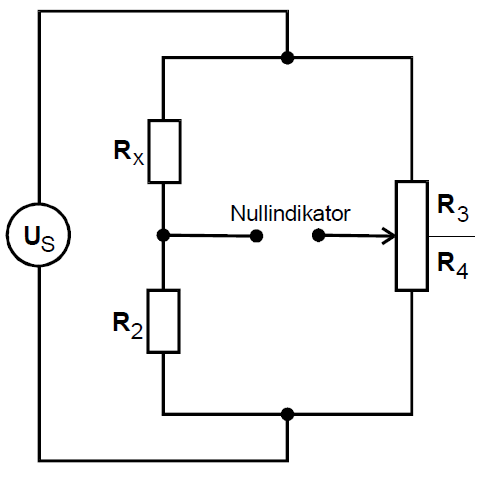
\includegraphics[width=\textwidth]{wheaton_bs.png}
\caption{Wheaton'sche Brückenschaltung}
\label{fig:wheaton}
\end{figure}
Diese Schaltung kann sowohl mit Gleichstrom, als auch mit Wechselstrom betrieben werden, da sie ausschließlich
ohm'sche Widerstände enthält. 
Aus [eq2] folgt für $R_x$:
\begin{equation}
\label{eqn:wheaton}
 R_x = R_2 \frac{R_3}{R_4}
\end{equation}

$\frac{R_3}{R_4}$ ist dabei als Potentiometer anzusehen, mit dem das Verhältnis zwischen $R_3$ und $R_4$ 
variiert werden kann. 

\subsubsection{Kapazitätsmessbrücke}
\begin{figure}
\centering
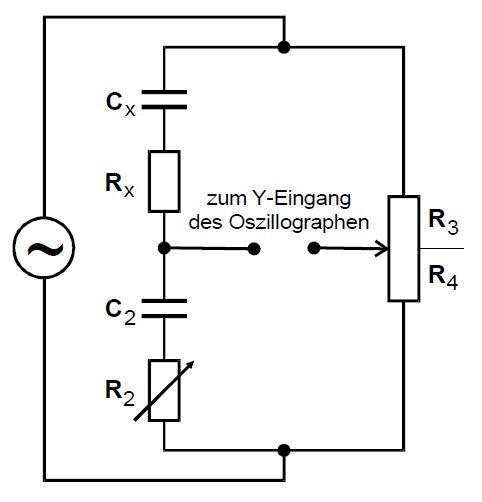
\includegraphics[width=\textwidth]{kondensator_bs.png}
\caption{Kapazitätsmessbrücke}
\label{fig:kapa}
\end{figure}
Wie in hier zu sehen ist, unterscheidet sich dieser Aufbau von \ref{fig:wheaton} durch 
einen Kondenstator unbekannter Kapazität, der anstelle des ohm'schen Widerstands verbaut ist, und einen zweiten
bekannten Kondensators, der vor $R_2$ geschaltet ist. 
Ein Kondenstator hat in der 
Realität die Eigenschaft, dass er beim Speichern elektrischer Energie einen Teil dieser in Wärmeenergie umwandelt
(analog zum ohm'schen Widerstand),
wodurch als Ersatzschaltbild für $C_x$ zusätzlich ein $R_x$ eingezeichnet wird. 
Dadurch ergibt sich in diesem Fall für den Widerstand des Kondensators $ Z_R$ = $R - \frac{i}{\omega C}$
Für $R_x$ und $C_x$ gilt dann 
\begin{equation}
\label{eqn:kapa1}
  R_x = R_2 \frac{R_3}{R_4} 
\end{equation}
 \quad und
\begin{equation}
\label{eqn:kapa2}
   C_x = C_2 \frac{R_4}{R_3} 
\end{equation}


$R_2$ ist hierbei variabel, um die Phasenverschiebung, die durch $R_x$ zustande kommt, ausgleichen zu können.
Hat der Kondensator nur sehr geringe dielektrische Verluste, so ist ein Einbau von $R_2$ nicht notwendig, 
da dann bis zu Frequenzen von etwa $10^4\si{\hertz}$ $R_x \ll \frac{1}{\omega C}$ und 
$R_2 \approx 0$ ist.

\subsubsection{Induktivitätsmessbrücke}

\begin{figure}
\centering
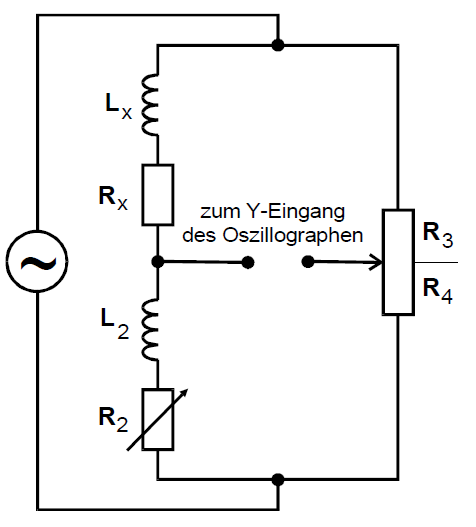
\includegraphics[width=\textwidth]{spule_bs.png}
\caption{Induktionsmessbrücke}
\label{fig:spule}
\end{figure}
Diese Schaltung funktioniert grundsätzlich analog zur Kapazitätsmessbrücke, mit dem Unterschied, dass 
\begin{equation*}
    Z_L = R - i\omega L
\end{equation*}
ist. Dadurch ist die Induktivität über \begin{equation}
\label{eqn:induk}
    L_x = L_2 \frac{R_3}{R_4}
\end{equation} beschrieben.

Die Verslustleistung von $L_2$ sollte dabei so klein wie möglich sein, da der Wirkwiderstand in diesem Abschnitt
der Masche
ausschließlich aus $R_2$ bestehen sollte. In der Realität ist dies, vor allem bei niedrigen Frequenzen, nur schwierig 
zu erreichen. Aus diesem Grund ist es oft sinnvoller, die Induktivität einer Spule durch eine Maxwell-Brücke zu 
bestimmen, wie sie im nächsten Teilabschnitt beschrieben ist.

\subsubsection{Maxwell-Brücke}

\begin{figure}
\centering
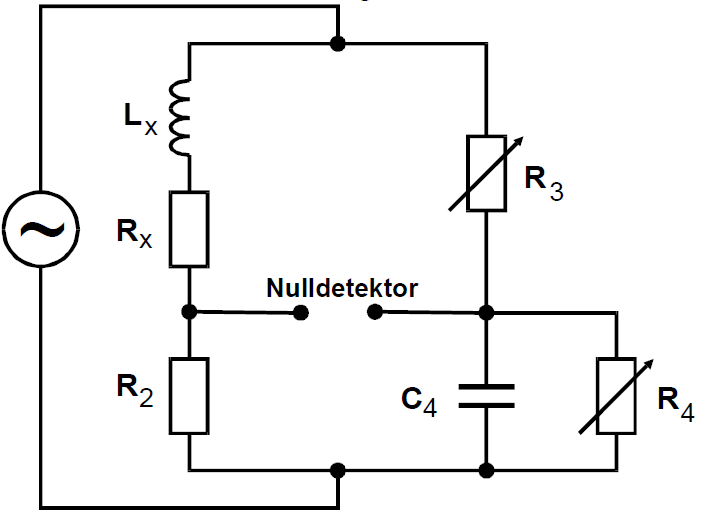
\includegraphics[width=\textwidth]{maxwell_bs.png}
\caption{Maxwell'sche Brückenschaltung}
\label{fig:maxwell}
\end{figure}
Die Abgleichelemente entalten hierbei keine bekannte Spule der Induktivität $L_2$, wodurch das Problem der 
standardmäßigen Induktivitätsmessbrücke aufgehoben wird. Stattdessen wird hier ein verlustarmer Kondenstator
der Kapazität $C_4$ mit einem, wie der Skizze zu sehen ist, leicht variiertem Aufbau verwendet. Die dabei
in Wärme umgewandelte Energie ist in diesem Fall einfacher gering zu halten, wodurch das Messen von $L_x$
im Regelfall präziser gelingt.

$Z_L$ ist gleich, wie bei der Induktivitätsmessbrücke, über die Kirchhoff'schen Gesetze folgt daraus für
diesen Aufbau \begin{equation}
\label{eqn:maxwell}
    L_x = R_2 R_3 C_4
\end{equation}

\subsubsection{Wien-Robinson-Brücke}
\label{sec:wien}
\begin{figure}
\centering
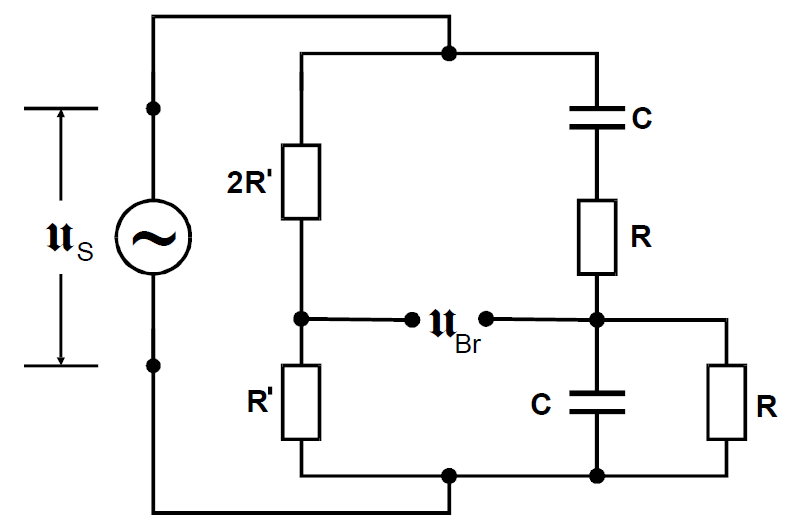
\includegraphics[width=\textwidth]{wien_robinson_bs.png}
\caption{Wien-Robinson-Brücke}
\label{fig:wien}
\end{figure}
Mit diesem Aufbau ist die frequenzabhängige Brückenspannung $U_{\text{Br}}$ zu bestimmen. Das Spannungsverhältnis
zwischen der Speisespannung $U_{\text{S}}$ und $U_{\text{Br}}$ lässt sich durch \begin{equation}
    \left|\frac{U_{\text{Br}}}{U_{\text{S}}}\right|^2 = \frac{1}{9}\frac{(\omega^2 R^2 C^2 -1)^2}{\bigl (1- \omega^2 R^2 C^2\bigr)^2 + 9\omega^2 R^2 C^2} 	
\end{equation}
Der Term wird null, wenn \begin{equation}
    \omega_0 = \frac{1}{RC}
\end{equation} ist. Daher wird das Frequenzverhältnis $\Omega$ := $\frac{\omega}{\omega_0}$ definiert, woraus für das
Spannungsverhältnis \begin{equation}
\label{eqn:u}
    \left|\frac{U_{\text{Br}}}{U_{\text{S}}}\right|^2 = \frac{1}{9}\frac{(\Omega^2 -1)^2}{(1- \Omega^2)^2 + 9\Omega^2}
\end{equation}

Dieses Spannungsverhältnis als $U_{\text{v}}$ wird für die später einfachere Referenzierzung zu
\begin{equation}
   U_{\text{v}}\coloneq \left|\frac{U_{\text{Br}}}{U_{\text{S}}}\right| = \sqrt{\frac{1}{9}\frac{(\Omega^2 -1)^2}{(1- \Omega^2)^2 + 9\Omega^2}}
\end{equation}
umgeformt und definiert.


Die Wien-Robinson-Brücke dient also Sperrfilter. Aus einem kontinuierlichen Frequenzspektrum können damit 
Schwingungen der Frequenz $\omega_0$ entfernt werden. Schwingungen, deren Frequenzen in der Umgebung von 
$\omega_0$ liegen, werden dabei abgeschwächt. Je geringer deren Frequenzen von $\omega_0$ abweichen, desto 
stärker ist diese Abschwächung. 

Darüber hinaus kann mit diesem Aufbau ein Klirrfaktor $k$ gemessen werden. Dieser beschreibt ein Verhältnis der 
Oberwellen zur Grundwelle einer Sinusschwingung. Eine perfekte Sinusschwingung enthält keine Oberwellen, wodurch deren 
Klirrfaktor null wird. In der Realität ist dies jedoch nur sehr schwierig zu erreichen. Die Qualität eines Sinusgenerators
kann daher über den Wert des Klirrfaktors bestimmt werden, der geringer wird, je besser genauer die Sinusschwingung ist, 
d.h. je geringer die Oberwellen von der Grundwelle abweichen. Der Klirrfaktor lässt sich im Allgemeinen über folgende
Formel angeben: \begin{equation}
    \label{eqn:k}
    k = \sqrt{\frac{\sum_{i=2}^N {U_i}^2}{U_1}}
\end{equation}
$U_1$ ist die Amplitude der Grundwelle und $U_i$ sind jeweils die Amplituden der insgesamt $n$ Oberwellen.






